%!TEX root = ../thesis.tex
%*******************************************************************************
%****************************** Third Chapter **********************************
%*******************************************************************************
\chapter{Diseño Conceptual}

% **************************** Define Graphics Path **************************
\ifpdf
    \graphicspath{{Chapter3/Figuras/}{Chapter3/Figs/PDF/}{Chapter3/Figs/}}
\else
    \graphicspath{{Chapter3/Figs/Vector/}{Chapter3/Figs/}}
\fi

\section{Requerimientos del sistema}
Uno de los requerimientos principales del sistema es el uso de una red de sensores modular y sencilla de instalar en distintos tipos de vehículos. Esto se explica fácilmente debido a que este sistema esta orientado a ser usado en el sistema de transporte público en Lima, el cual tiene una gran variedad y un gran número de vehículos. El sistema, entonces, debe ser adaptable a cualquiera de estos vehículos y no contar con un tiempo de instalación elevado.

También se tiene como requerimiento un grado de precisión alto en el reconocimiento de estilos y eventos de conducción. Esto es necesario debido a que este sistema se usará para monitorizar y mejorar la conducta de conducción de los choferes del servicio de transporte público. Los datos arrojados por este sistema necesitan ser confiables.

Por último, se necesita también de una adecuada infraestructura que permita que el sistema funcione en linea, entregando feedback al conductor, aún si se presentan condiciones como la falta temporal de conexión a Internet. Este requerimiento será importante al considerar donde realizar el procesamiento de los datos (dentro de un sistema embebido en cada vehículo o usando un servidor).


\begin{table}[htbp!]
  \caption{Lista de Requerimientos página 1.}
  \label{diag:3.1}
  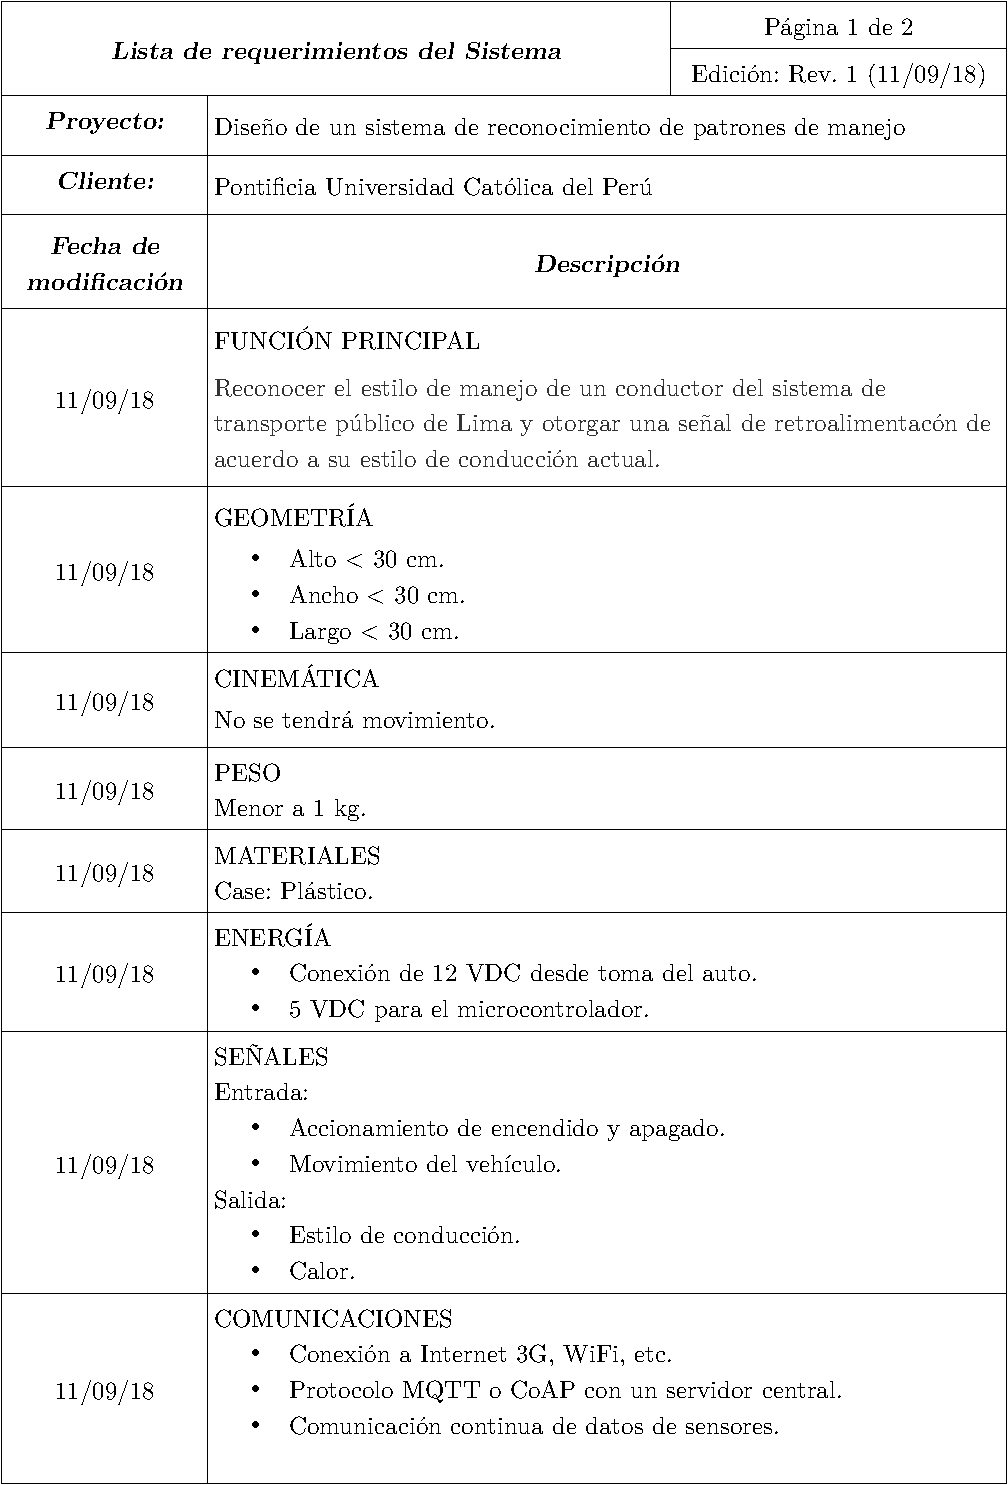
\includegraphics[width=1.05\linewidth]{Tab1.pdf}
\end{table}

\begin{table}[htbp!]
  \caption{Lista de Requerimientos página 2.}
  \label{diag:3.2}
  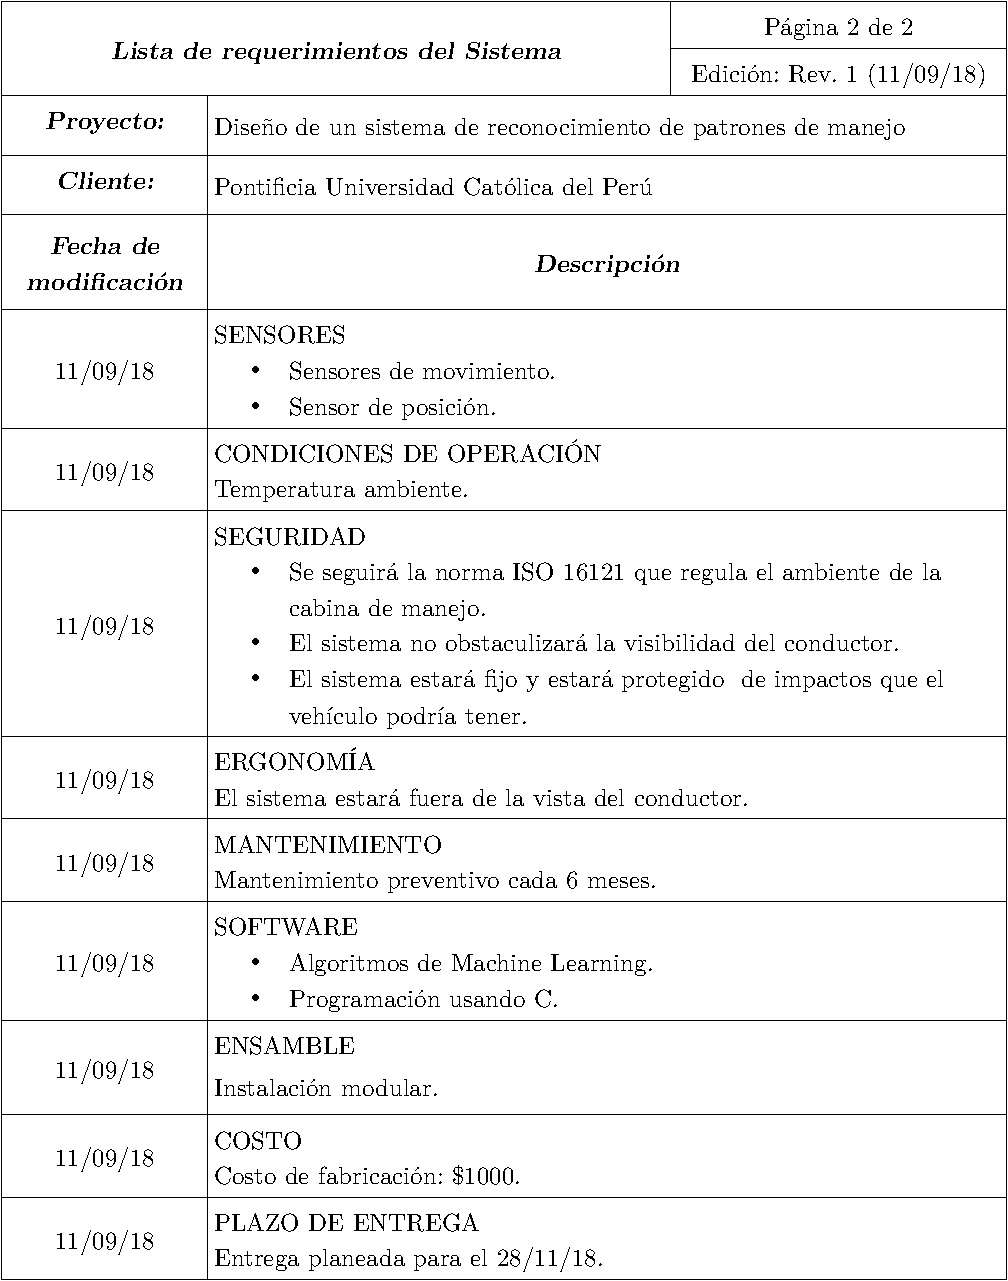
\includegraphics[width=1.05\linewidth]{Tab2.pdf}
\end{table}

\newpage

\section{Modelo Black Box}
En la Fig~\ref{fig:3.1} se puede observar el modelo de Black Box o Caja Negra del sistema. En este modelo se pueden apreciar con mayor claridad las entradas y salidas del sistema

\begin{figure}[htbp!]
\centering
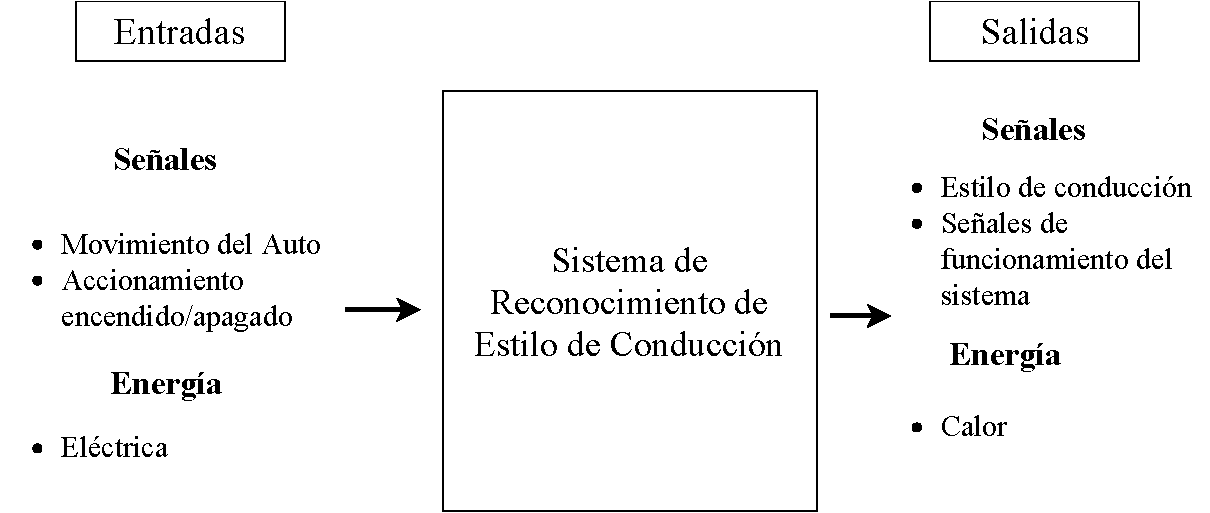
\includegraphics[width=\textwidth]{Fig1.pdf}
\caption{Modelo de Black Box del sistema.}
\label{fig:3.1}
\end{figure}


El sistema estará conectado al auto, de donde obtendrá la energía necesaria para funcionar. Debido a que el enfoque del sistema es ahorrar energía, su consumo debe ser reducido.

Además de recibir la energía, este sistema procesará el movimiento del auto usando sensores obteniendo así toda la información necesaria para caracterizar el estilo de conducción del usuario. El estilo de conducción será obtenido a través del procesamiento de la información de los sensores y será representado como una señal de retroalimentación al usuario.

\section{Estructura de Funciones}

\begin{sidewaysfigure}[htbp!]
\centering
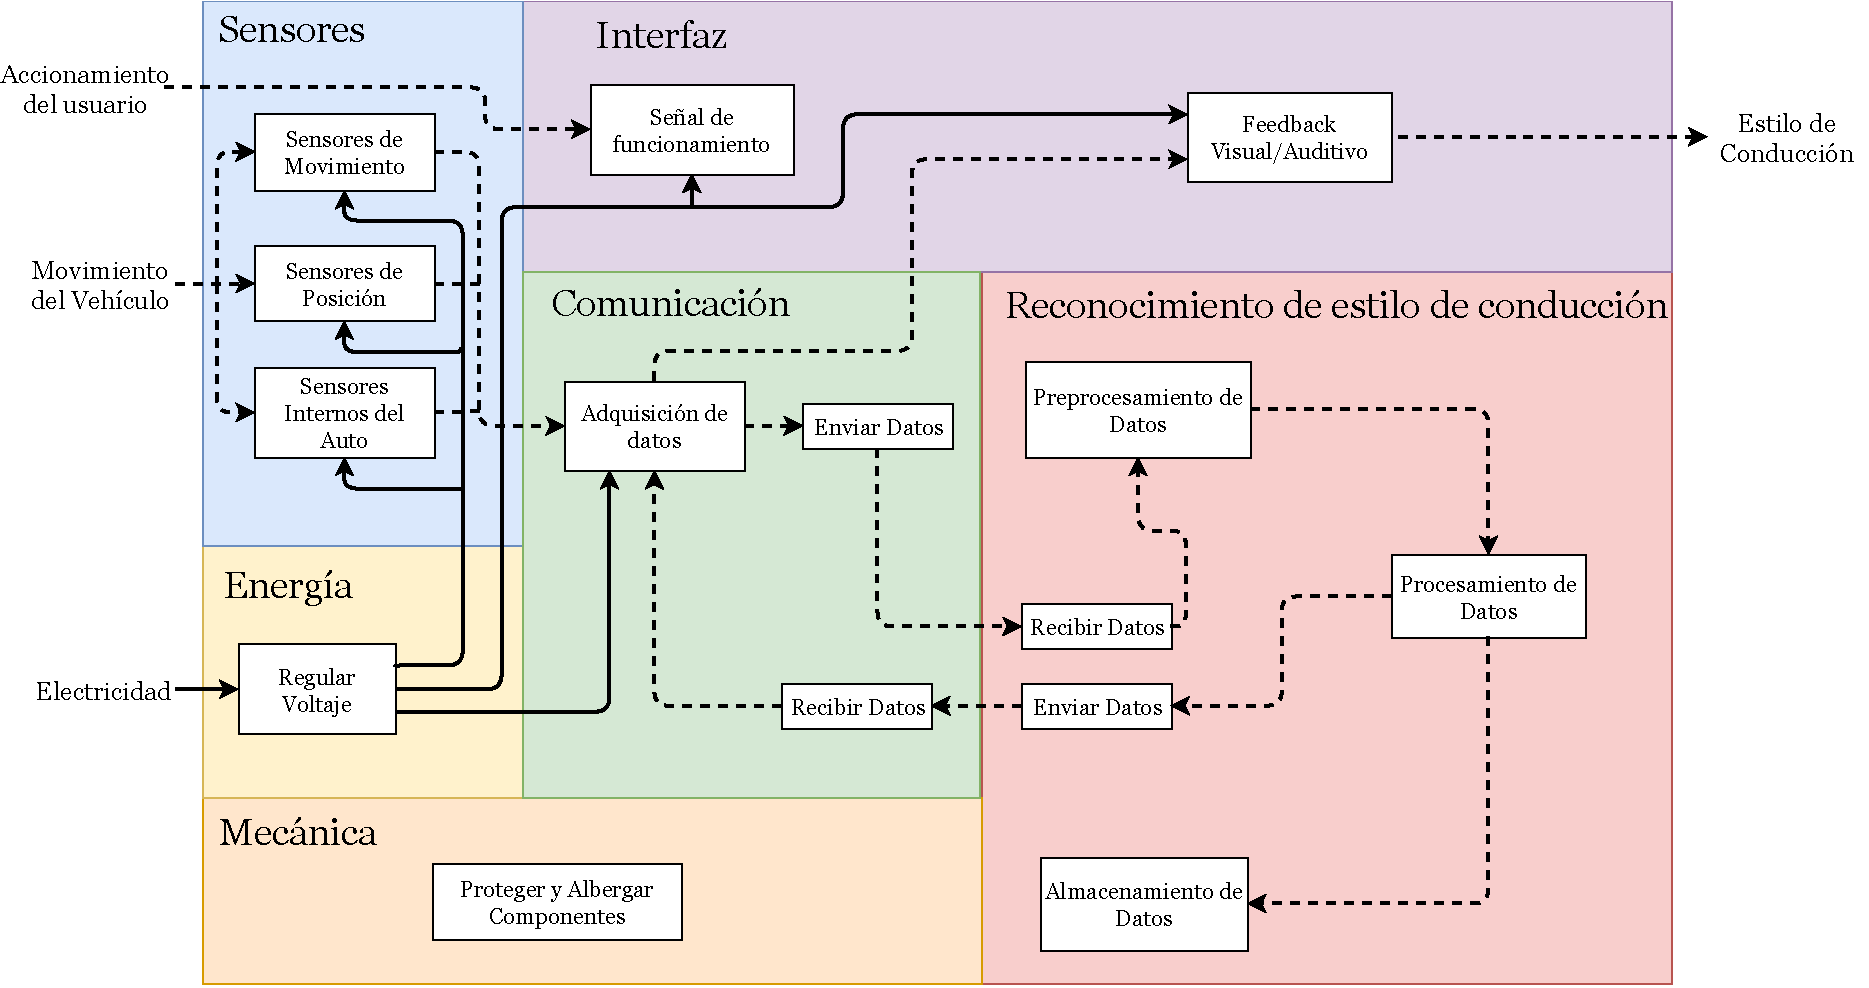
\includegraphics[width=\textwidth]{Tab3.pdf}
\caption{Estructura de Funciones.}
\label{fig:3.2}
\end{sidewaysfigure}

La estructura de funciones del sistema se puede apreciar en la Fig~\ref{fig:3.2}. Para el elaboramiento de esta se han considerado 7 Dominios: Mecánica, Energía, Sensores, Procesamiento, Comunicación, Reconocimiento del estilo de conducción e Interfaz.

Se describirá a continuación cada uno de estos dominios para así obtener una visión general del funcionamiento total del sistema.

\subsection{Dominio Mecánico}
En este dominio (Fig~\ref{fig:3.3}) se encuentra la  función de proteger y albergar todos los componentes del sistema. Esta función hace referencia al case que encapsulará todos los elementos. Además, se debe tener en cuenta que la velocidad relativa entre el vehículo y el sistema debe ser nula para que las medidas de los sensores sean precisas. Es por eso que se tiene como otra función el sujetar los componentes.


\begin{figure}[htbp!]
\centering
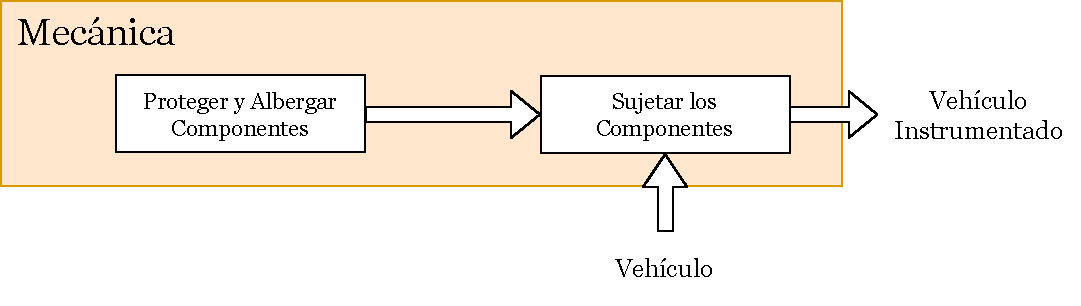
\includegraphics[width=\textwidth]{mec.pdf}
\caption{Dominio Mecánico de la estructura de funciones.}
\label{fig:3.3}
\end{figure}

\subsection{Dominio de Energía}
Este dominio (Fig~\ref{fig:3.4}) cumplirá la función de obtener la energía eléctrica necesaria para el funcionamiento del sistema y regular el voltaje, entregándole a cada Dominio esta energía según sus requerimientos específicos. Los módulos que recibirán la energía serán los de Procesamiento, Sensores e Interfaz.

\begin{figure}[htbp!]
\centering
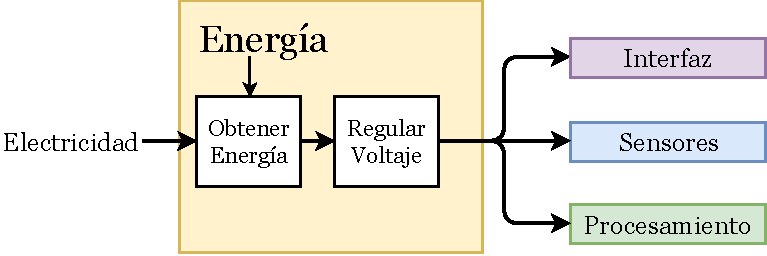
\includegraphics[width=0.8\textwidth]{elec.pdf}
\caption{Dominio Eléctrico de la estructura de funciones.}
\label{fig:3.4}
\end{figure}


\subsection{Dominio de Sensores}
Este dominio (Fig~\ref{fig:3.5}) realizará la función de recibir la información del movimiento del vehículo, de su posición y de obtener los parámetros internos del auto. Luego transmitirá esta información al dominio de Procesamiento que manejará todos los datos.

\begin{figure}[htbp!]
\centering
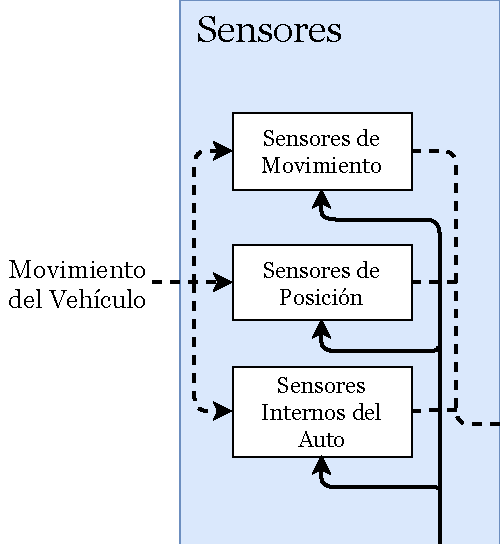
\includegraphics[width=0.7\textwidth]{sens.pdf}
\caption{Dominio de Sensores de la estructura de funciones.}
\label{fig:3.5}
\end{figure}


\subsection{Dominio de Comunicación}
En este módulo (Fig~\ref{fig:3.6}) se recopilaran los datos que se manipularon el el Dominio de Procesamiento y se entregarán al dominio de Reconocimiento de Estilo de Conducción.

\begin{figure}[htbp!]
\centering
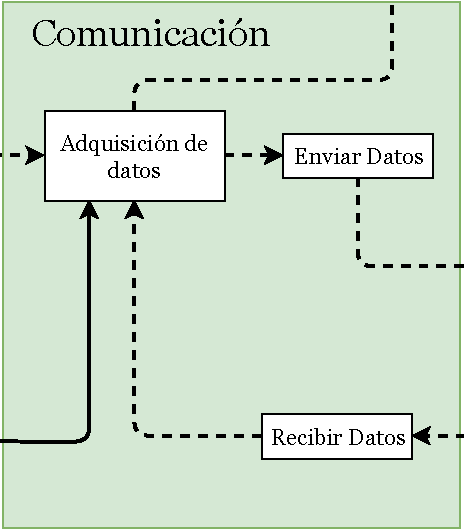
\includegraphics[width=0.9\textwidth]{com.pdf}
\caption{Dominio de Comunicación de la estructura de funciones.}
\label{fig:3.6}
\end{figure}

\subsection{Dominio de Procesamiento}
Este dominio (Fig~\ref{fig:proces}) realizará la función de recibir la información del dominio de sensores y encapsular los datos para que el dominio de comunicación pueda enviarlos. Luego recibe los datos a través del dominio de comunicación y se encarga de generar la señal de retroalimentación y enviársela al dominio de interfaz.

\begin{figure}[htbp!]
\centering
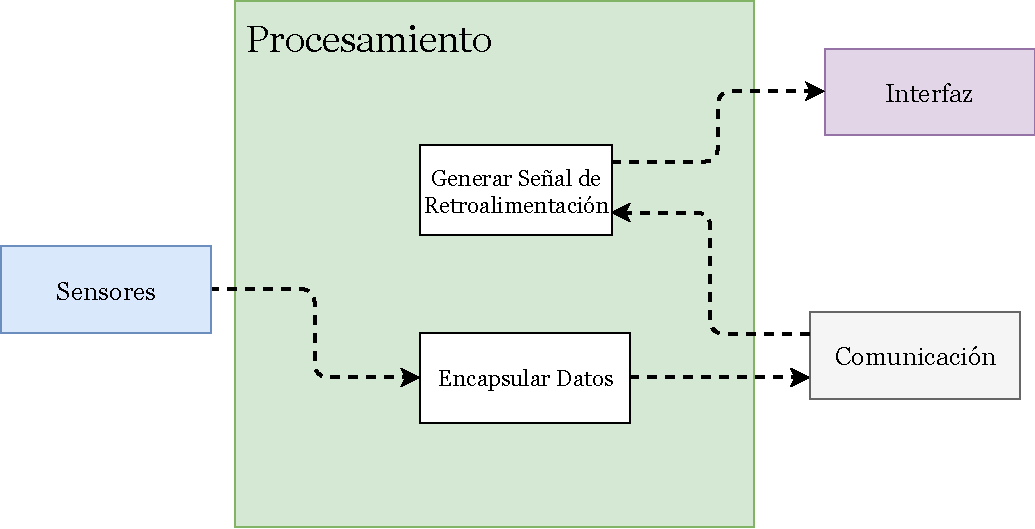
\includegraphics[width=0.8\textwidth]{proc.pdf}
\caption{Dominio de Procesamiento de la estructura de funciones.}
\label{fig:proces}
\end{figure}

\subsection{Dominio de Interfaz}
Este dominio (Fig~\ref{fig:int}) realizará la función de recibir la señal de retroalimentación del dominio de Procesamiento y usarla para mostrarle al usuario la retroalimentación (de forma visual, auditiva o háptica).

\begin{figure}[htbp!]
\centering
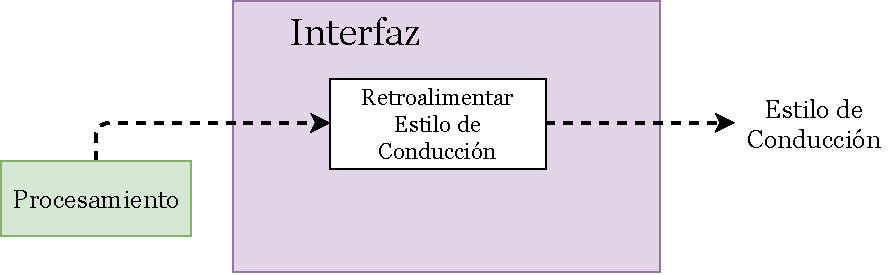
\includegraphics[width=0.8\textwidth]{int.pdf}
\caption{Dominio de Interfaz de la estructura de funciones.}
\label{fig:int}
\end{figure}

\subsection{Dominio de Reconocimiento de Estilo de Conducción}
En este Dominio se realizará el reconocimiento del estilo de conducción usando . Para alcanzar esto se los datos atraviesan 3 etapas. La etapa de segmentación de datos, en la que se dividen en

realizará un preprocesamiento de la data para luego procesarla usando algoritmos de machine learning.

\begin{figure}[htbp!]
\centering
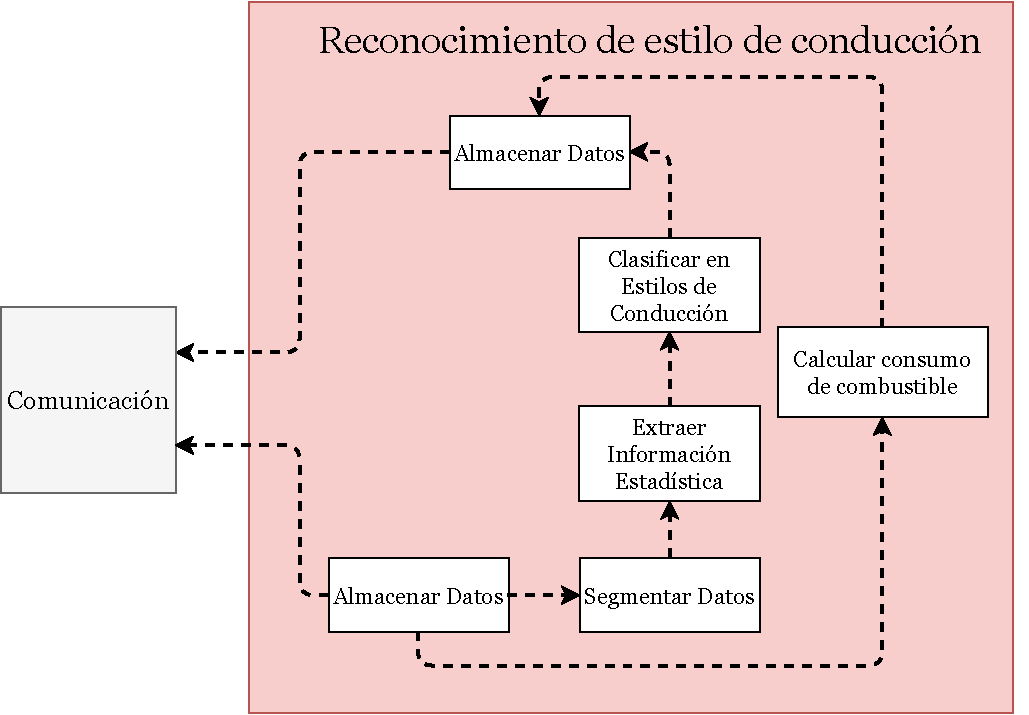
\includegraphics[width=0.8\textwidth]{rec.pdf}
\caption{Dominio de Reconocimiento de Estilo de Conducción de la estructura de funciones.}
\label{fig:3.7}
\end{figure}


\section{Matriz morfológica por dominio}
En esta sección se propondrán la Matriz morfológica por cada dominio de la estructura de funciones mostrada anteriormente. Cada función tendrá distintas alternativas portadores de solución que al combinarse formarán una solución completa.

\subsection{Dominio Mecánico}
Se presenta a continuación la matriz morfológica del dominio mecánico en la Tabla~\ref{diag:morf_mec} y la descripción de los conceptos de solución propuestos en la Tabla~\ref{diag:sol_mec}.
\begin{table}[htbp!]
  \caption{Matriz Morfológica del Dominio Mecánico}
  \label{diag:morf_mec}
  \centering
  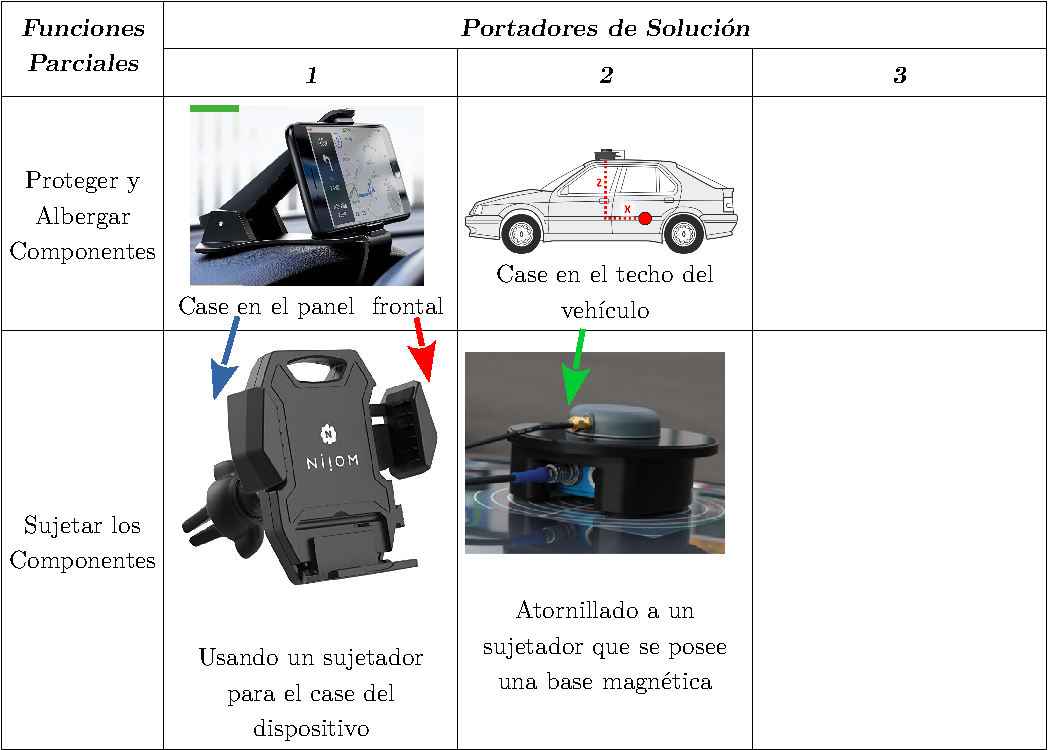
\includegraphics[width=0.9\linewidth]{morf_mec.pdf}
\end{table}

\newpage
\begin{table}[htbp!]
  \caption{Conceptos de solución mecánicos propuestos}
  \label{diag:sol_mec}
  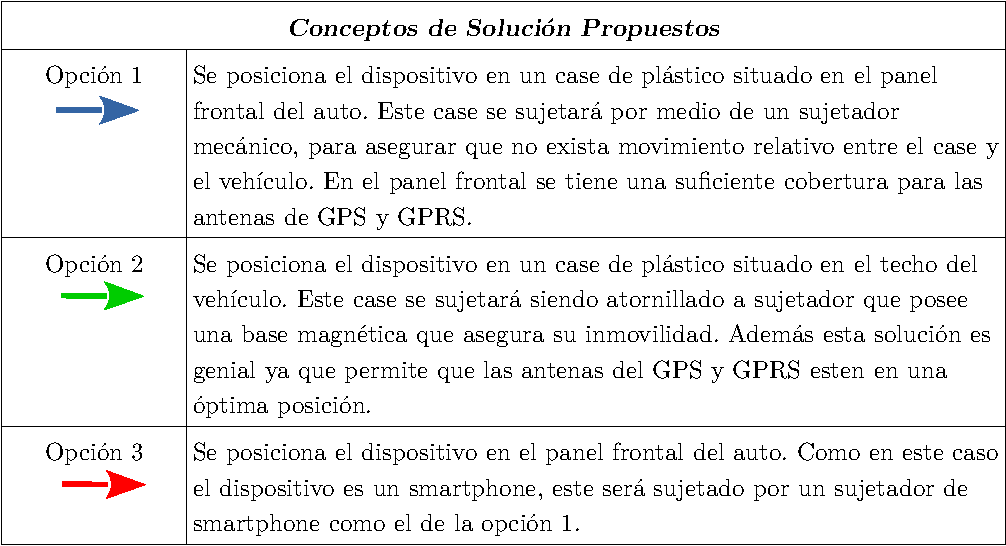
\includegraphics[width=\linewidth]{sol_mec.pdf}
\end{table}


\subsection{Dominio Energético}
Se presenta a continuación la matriz morfológica del dominio eléctrico en la Tabla~\ref{diag:morf_elec} y la descripción de los conceptos de solución propuestos en la Tabla~\ref{diag:sol_elec}.

\begin{table}[htbp!]
  \caption{Matriz Morfológica del Dominio Energético}
  \label{diag:morf_elec}
  \centering
  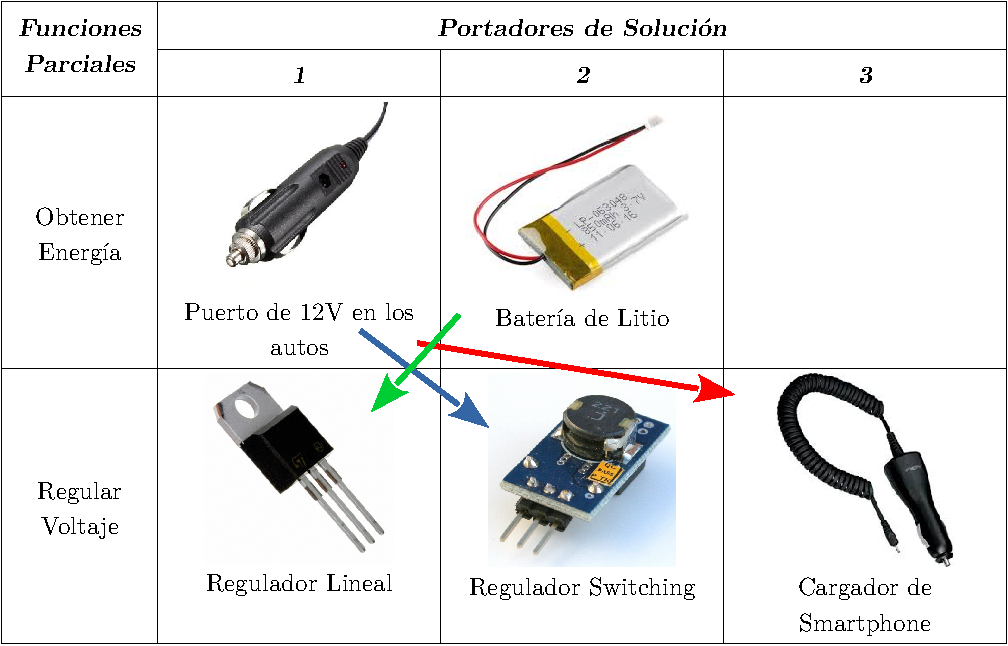
\includegraphics[width=0.9\linewidth]{morf_elec.pdf}
\end{table}

%\newpage

\begin{table}[htbp!]
  \caption{Conceptos de solución eléctricos propuestos}
  \label{diag:sol_elec}
  \centering
  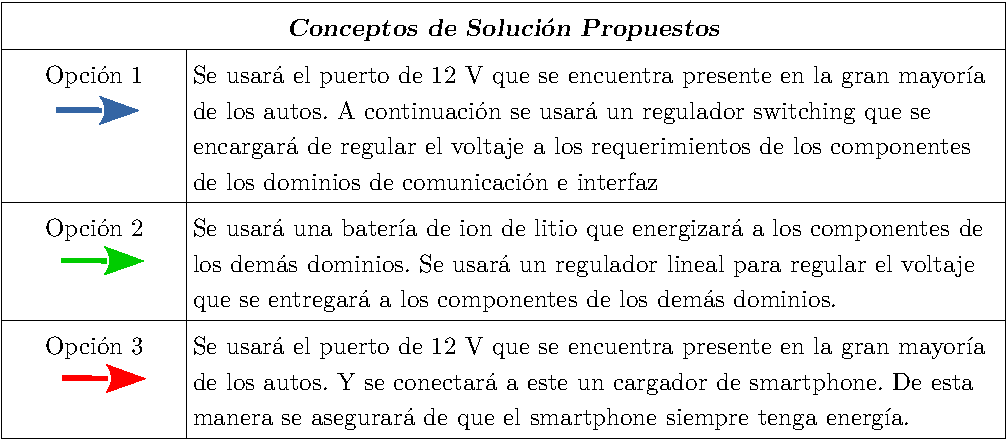
\includegraphics[width=\linewidth]{sol_elec.pdf}
\end{table}

\subsection{Dominios de Procesamiento y de Comunicación}
Se presenta a continuación la matriz morfológica del dominio de comunicación en la Tabla~\ref{diag:morf_com} y la descripción de los conceptos de solución propuestos en la Tabla~\ref{diag:sol_com}.

\begin{table}[htbp!]
  \caption{Matriz Morfológica de los Dominios de Procesamiento y Comunicación}
  \label{diag:morf_com}
  \centering
  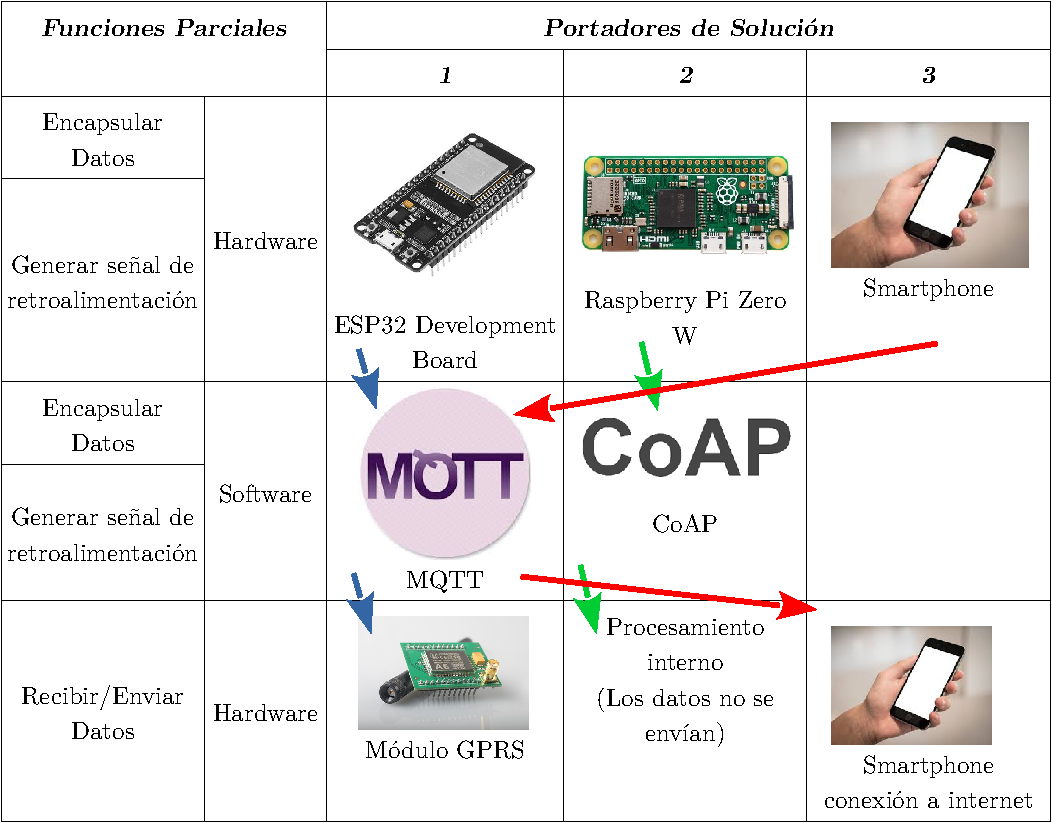
\includegraphics[width=\linewidth]{morf_com.pdf}
\end{table}

\begin{table}[htbp!]
  \caption{Conceptos de solución propuestos del dominio de comunicación}
  \label{diag:sol_com}
  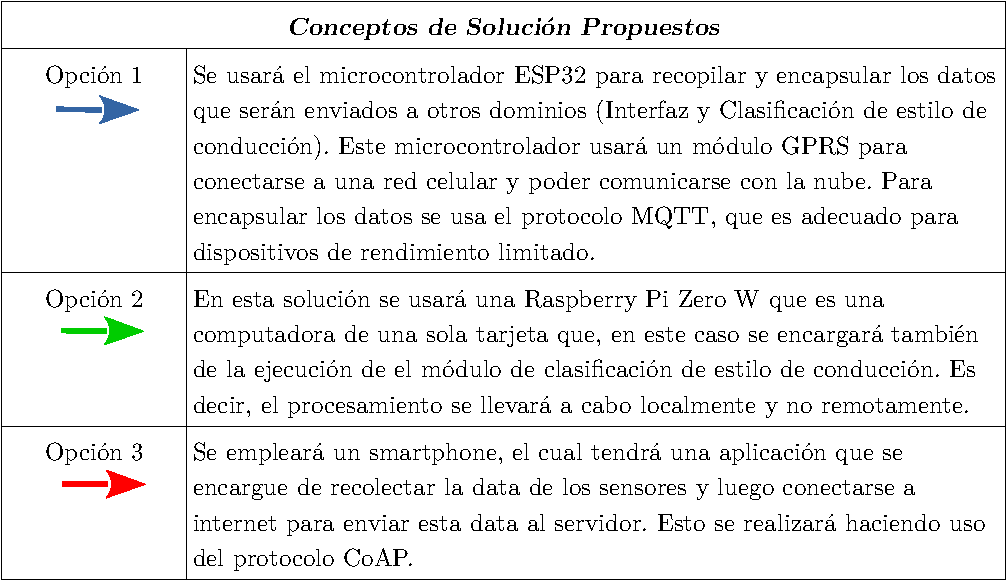
\includegraphics[width=\linewidth]{sol_com.pdf}
\end{table}

\subsection{Dominio de Sensores}
Se presenta a continuación la matriz morfológica del dominio de sensores en la Tabla~\ref{diag:morf_sens} y la descripción de los conceptos de solución propuestos en la Tabla~\ref{diag:sol_sens}.
\begin{table}[htbp!]
  \caption{Matriz Morfológica del Dominio de Sensores}
  \label{diag:morf_sens}
  \centering
  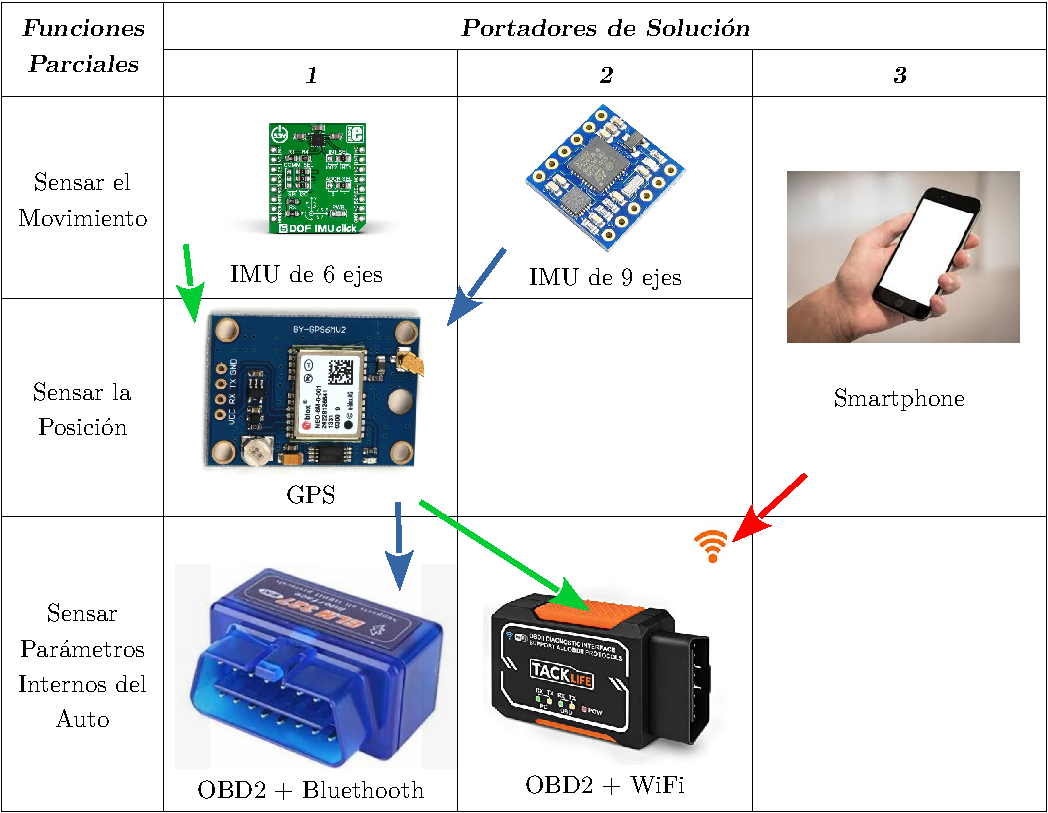
\includegraphics[width=0.9\linewidth]{morf_sens.pdf}
\end{table}

\newpage

\begin{table}[htbp!]
  \caption{Conceptos de solución propuestos del dominio de sensores}
  \label{diag:sol_sens}
  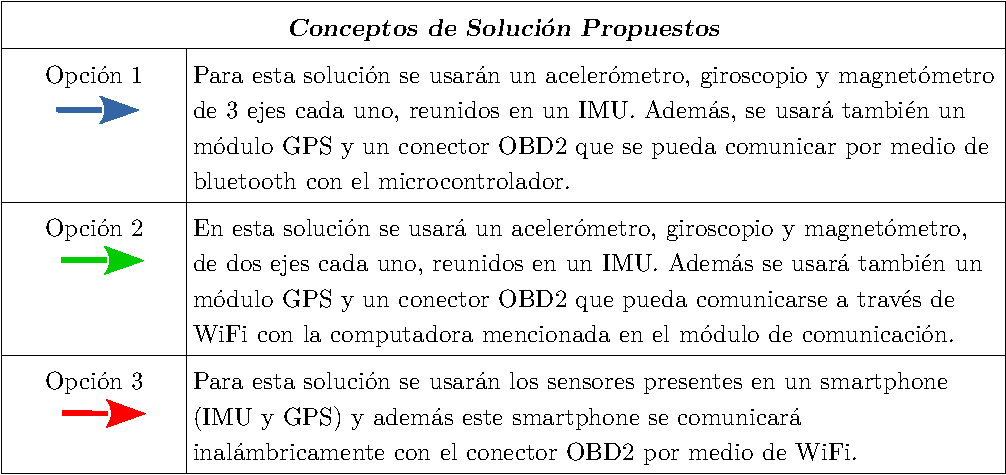
\includegraphics[width=\linewidth]{sol_sens.pdf}
\end{table}


\subsection{Dominio de Interfaz}
Se presenta a continuación la matriz morfológica del dominio de interfaz en la Tabla~\ref{diag:morf_int} y la descripción de los conceptos de solución propuestos en la Tabla~\ref{diag:sol_int}.
\begin{table}[htbp!]
  \caption{Matriz Morfológica del Dominio de Interfaz}
  \label{diag:morf_int}
  \centering
  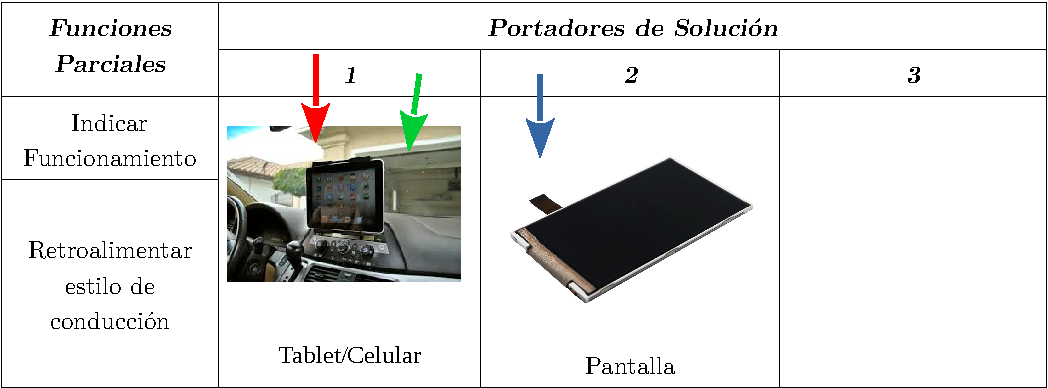
\includegraphics[width=\linewidth]{morf_int.pdf}
\end{table}

\begin{table}[htbp!]
  \caption{Conceptos de solución propuestos del dominio de interfaz}
  \label{diag:sol_int}
  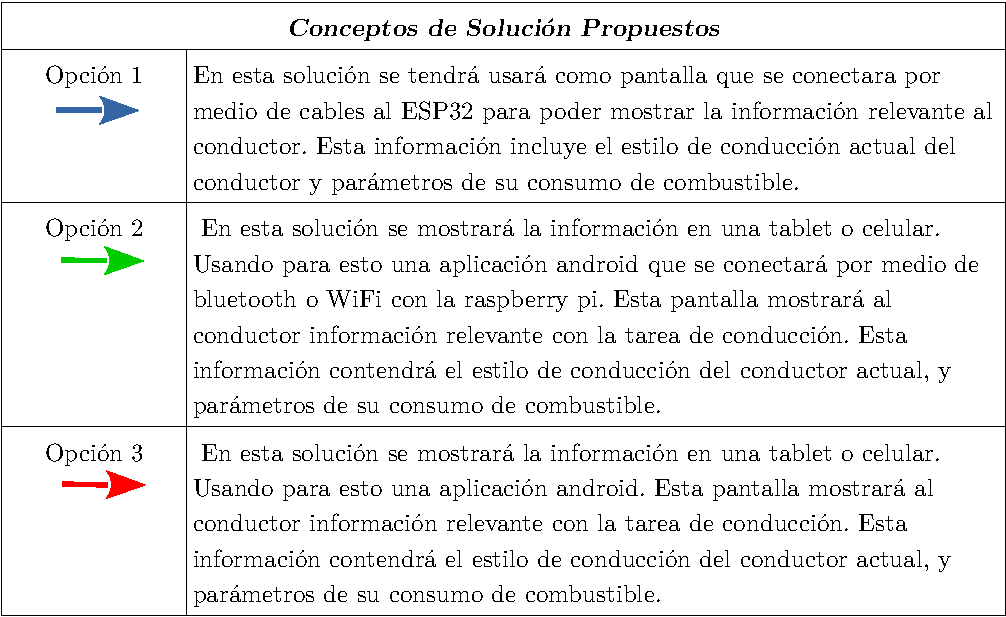
\includegraphics[width=\linewidth]{sol_int.pdf}
\end{table}

%\newpage

\subsection{Dominio de Reconocimiento de estilo de conducción}
Se presenta a continuación la matriz morfológica del dominio de reconocimiento de estilo de conducción en la Tabla~\ref{diag:morf_clas} y la descripción de los conceptos de solución propuestos en la Tabla~\ref{diag:sol_clas}.
\begin{table}[htbp!]
  \caption{Matriz Morfológica de Reconocimiento de estilo de conducción}
  \label{diag:morf_clas}
  \centering
  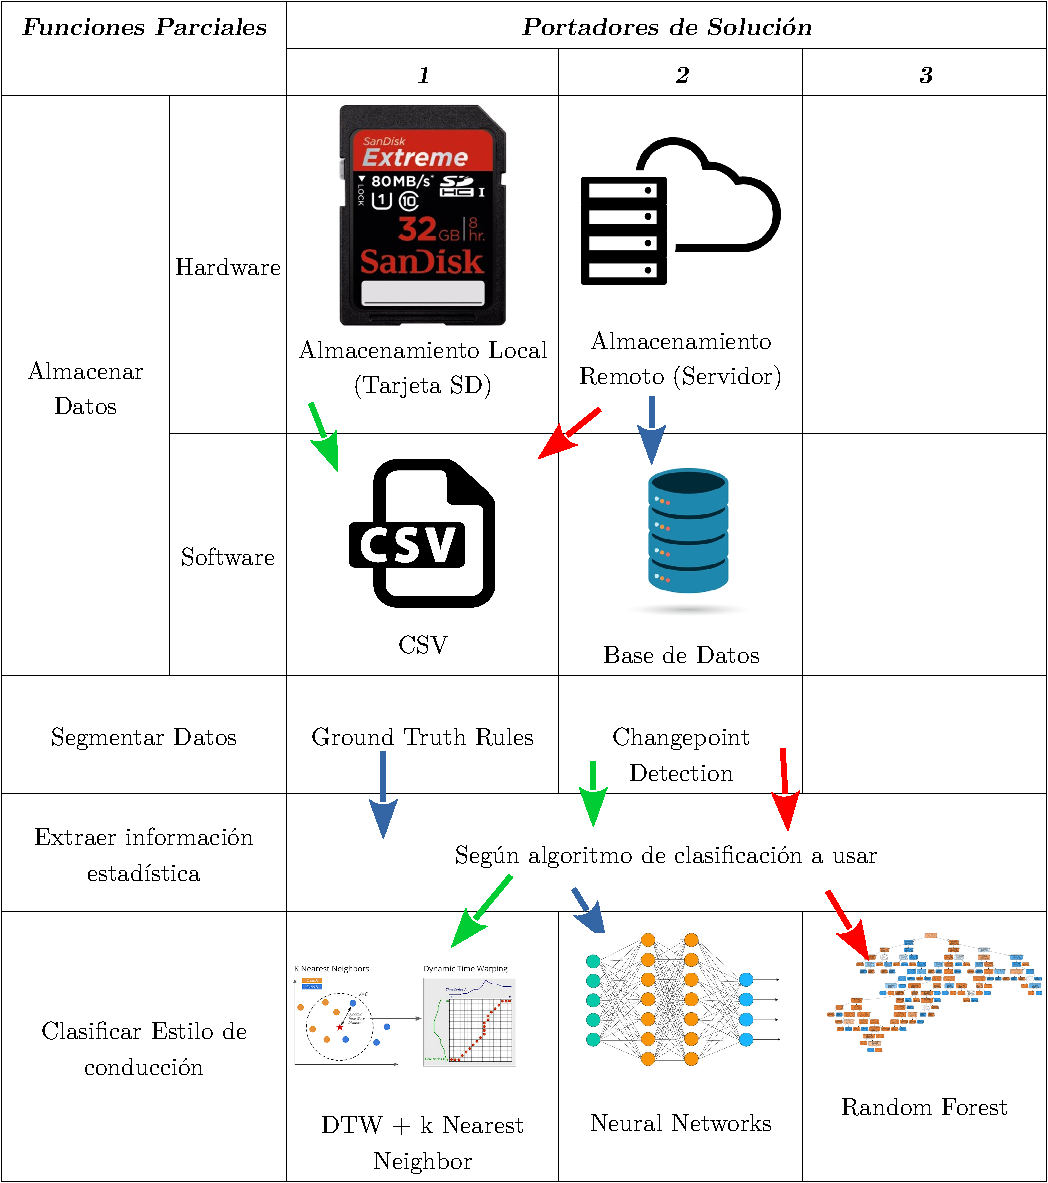
\includegraphics[width=\linewidth]{morf_clas.pdf}
\end{table}
\
\begin{table}[htbp!]
  \centering
  \caption{Conceptos de solución propuestos del dominio de reconocimiento de estilo de conducción}
  \label{diag:sol_clas}
  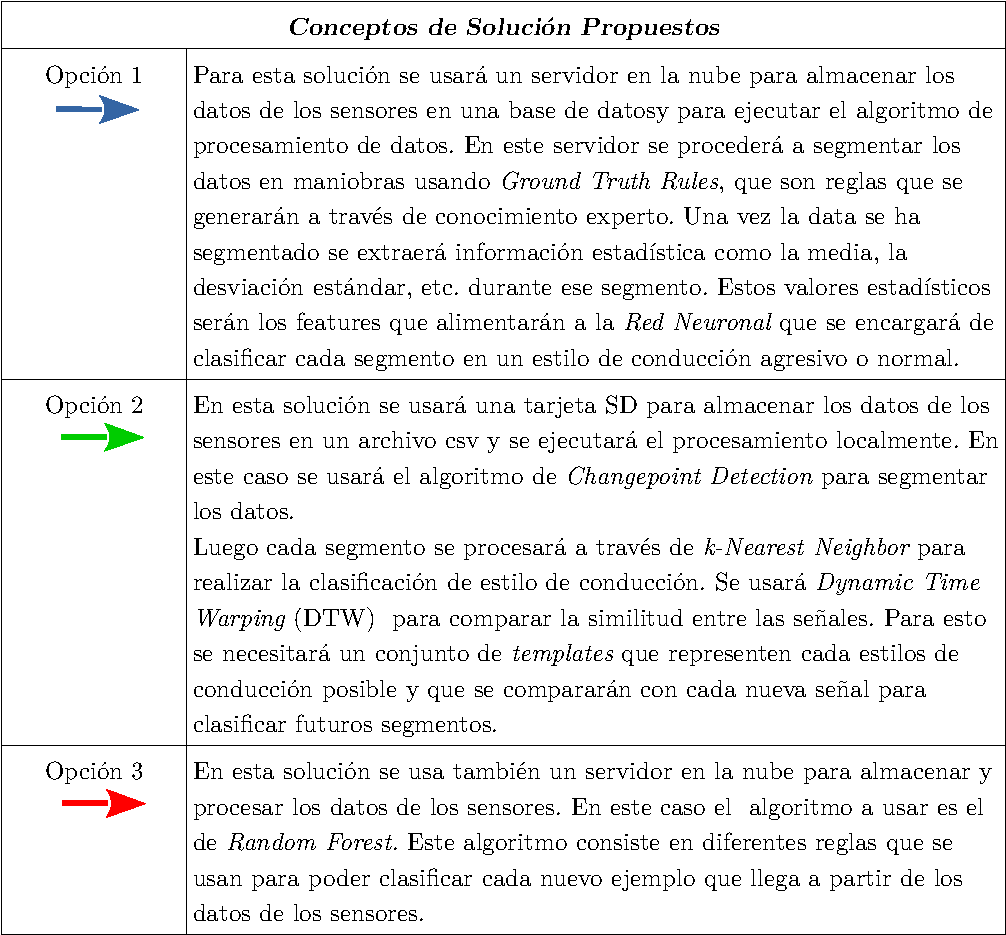
\includegraphics[width=\linewidth]{sol_clas.pdf}
\end{table}

\newpage

\section{Conceptos integrados de solución}
En la Tabla~\ref{diag:resumen} se puede observar un resumen de las soluciones escogidas por cada concepto de solución propuesto. Se describirán cada una de las soluciones para luego analizarlas con el fin de obtener la solución óptima.

\begin{table}[htbp!]
  \centering
  \caption{Conceptos de solución propuestos}
  \label{diag:resumen}
  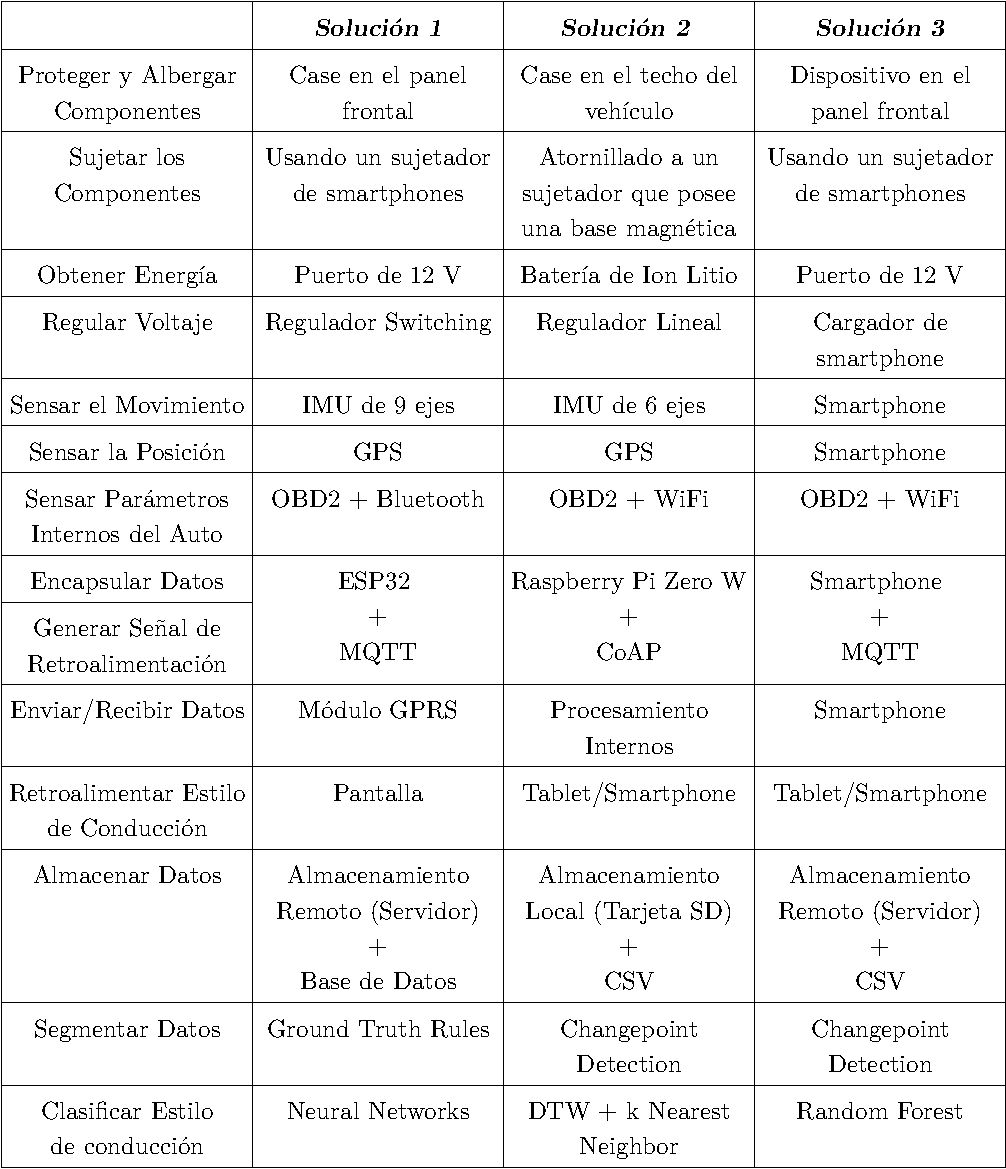
\includegraphics[width=0.9\linewidth]{mat_resumen.pdf}
\end{table}
\newpage

\subsection{Concepto integrado de solución 1}
El sistema se encuentra contenido en un case de plástico, que albergará todos los componentes electrónicos y que se sujetará usando un {\it phone holder} en el panel frontal del auto. Además, este sistema contará con una pantalla que estará posicionada de tal manera que el conductor pueda mirarla con facilidad. Este elemento será el que retroalimente el estilo de conducción al conductor.

El dispositivo se conectará a la toma de \SI{12}{V} y a través de un regulador switching se alcanzarán los \SI{3.3}{V} que necesita el ESP32 y los \SI{5}{V} que necesitan algunos de los módulos.
Estos módulos consisten en: Un acelerómetro de 3 ejes, un giroscopio de 3 ejes, un magnetómetro de 3 ejes (IMU), un módulo GPS y un módulo GPRS.

El conector OBD2 es el único módulo que no será energizado por el regulador switching, debido a que se conectará al puerto OBD2 del auto y obtendrá energía por este mismo medio. Este conector se comunicará por medio de bluetooth al microcontrolador y de esta manera obtendrá los parámetros internos del vehículo.

El microcontrolador entonces gestionará todo los datos recibidos y se encargará usar el protocolo MQTT para enviarlos. Usando el módulo GPRS que se conectará a internet, haciendo legar los datos hasta el servidor. Luego los datos se almacenarán en una base de datos y se procesarán allí.

El primer paso para procesar los datos es segmentarlos en periodos en los que se realiza determinada maniobra con un solo estilo de conducción. Esto se puede lograr a través de reglas antes predefinidas usando conocimiento experto. Estas reglas son llamadas {\it Ground Truth Rules}.

El segundo paso es analizar el segmento estadísticamente. Se definirán una serie de {\it features} que representen adecuadamente al segmento de datos. Estos features podrían ser: media, desviación estándar, máximo , mínimo, etc. Estos elementos serán las entradas de la {\it red neuronal} que ya ha sido entrenada previamente con una cantidad significativa de datos.

La red neuronal procesará las entradas y arrojará en la salida la clase a la que pertenece este segmento, pudiendo ser estilo de conducción agresivo o estilo de conducción normal. Una vez que se tiene el estilo de conducción clasificado, se procede a enviarlo de regreso hacia el microcontrolador. Este se encargará de recibir la clasificación y de acondicionar esta información para mostrarla en la pantalla presente en el vehículo. Esta pantalla mostrará el estilo de conducción reconocido y un estimado de el consumo de combustible actual si esta disponible.

El cálculo de consumo de combustible se realizará también en el servidor usando parte de los datos que provienen del módulo OBD2. Sin embargo,  esta información solo estará disponible si se tienen los parámetros adecuados desde el puerto OBD2 (Cada auto tiene disponibles diferentes parámetros).

\subsection{Concepto integrado de solución 2}
El sistema se encuentra contenido en un case de plástico, que albergará todos los componentes electrónicos y que se sujetará usando sujetador magnético en la parte superior del auto (techo). Además, este sistema contará con smartphone o tablet que este sujetada por un phone holder de tal manera que el conductor pueda mirarla con facilidad. Este elemento será el que retroalimente el estilo de conducción al conductor.

El dispositivo contará con una batería de ion litio con la que se encargará de obtener energía para su funcionamiento y a través de un regulador lineal se alcanzarán los \SI{5}{V} que necesita la raspberry pi zero w y algunos de los módulos. Estos módulos consisten en: Un acelerómetro de 2 ejes, un giroscopio de 2 ejes, un magnetómetro de 2 ejes (IMU de 6 ejes), un módulo GPS y un módulo GPRS.

El conector OBD2 es el único módulo que no será energizado por el regulador lineal, debido a que se conectará al puerto OBD2 del auto y obtendrá energía por este mismo medio. Este conector se comunicará por medio de WiFi a la raspberry y de esta manera obtendrá los parámetros internos del vehículo.

La raspberry entonces gestionará todo los datos recibidos y se encargará de procesarlos localmente. El primer paso para procesar los datos es segmentarlos en periodos en los que se realiza determinada maniobra con un solo estilo de conducción. Esto se puede lograr a través de un algoritmo llamado {\it changepoint detection} que analiza el comportamiento de las señales y trata de dividirlas en segmentos en donde su comportamiento sea lineal o cercano a lineal.

El segundo paso es analizar el segmento y clasificarlo usando el algoritmo de {\it k-NN}. Este algoritmo consiste en comparar el segmento obtenido con segmentos ejemplo que se tienen almacenados, y otorgarle la clase de acuerdo a los ejemplos que sean mas similares a este segmento.

El algoritmo arrojará entonces la clase a la que pertenece este segmento, pudiendo ser estilo de conducción agresivo o estilo de conducción normal. Una vez que se tiene el estilo de conducción clasificado, se procede a enviarlo en la tablet o celular presente en el vehículo para retroalimentar la información al conductor. En el smartphone o tablet existirá una aplicación que mostrará el estilo de conducción reconocido y un estimado de el consumo de combustible actual si esta disponible.

El cálculo de consumo de combustible se realizará en la raspberry pi usando parte de los datos que provienen del módulo OBD2. Sin embargo,  esta información solo estará disponible si se tienen los parámetros adecuados desde el puerto OBD2 (Cada auto tiene disponibles diferentes parámetros).

\subsection{Concepto integrado de solución 3}
En esta solución el sistema usará los sensores internos del smartphone para recopilar los datos necesarios, por lo que se requerirá un sujetador de smartphone para autos en el panel frontal del auto que este posicionado de tal manera que el conductor pueda mirarla con facilidad, ya que el smartphone también mostrará los datos obtenidos luego de la clasificación.

El dispositivo se conectará a la toma de \SI{12}{V} por medio del cargador de smartphone, para asegurarse de no perder energía y apagarse.

El conector OBD2 es el único módulo que no será energizado por el cargador de smartphone, debido a que se conectará al puerto OBD2 del auto y obtendrá energía por este mismo medio. Este conector se comunicará por medio de WiFi con el smartphone y de esta manera se obtendrán los parámetros internos del vehículo.

El smartphone entonces usará una aplicación android, que será la que gestionará todo los datos recibidos y se encargará usar el protocolo MQTT para enviarlos a un servidor remoto. Para esto se se conectará a internet usando 3G, 4G o la línea que se encuentre dispoible. Luego los datos se almacenarán en una base de datos y se procesarán en el servidor.

El primer paso para procesar los datos es segmentarlos en periodos en los que se realiza determinada maniobra con un solo estilo de conducción. Esto se puede lograr a través de un algoritmo llamado {\it changepoint detection} que analiza el comportamiento de las señales y trata de dividirlas en segmentos en donde su comportamiento sea lineal o cercano a lineal.

El segundo paso es usar el Random Forest para clasificar adecuadamente este segmento en un estilo de conducción agresivo o estilo de conducción normal. Una vez que se tiene el estilo de conducción clasificado, se procede a enviarlo de regreso hacia el smartphone. la aplicación, entonces,  se encargará de recibir la clasificación y de acondicionar esta información para mostrarla en la tablet o celular presente en el vehículo. Esta aplicación mostrará también un estimado de el consumo de combustible actual si este esta disponible.

El cálculo de consumo de combustible se realizará también en el servidor usando parte de los datos que provienen del módulo OBD2. Sin embargo,  esta información solo estará disponible si se tienen los parámetros adecuados desde el puerto OBD2 (Cada auto tiene disponibles diferentes parámetros).

\section{Evaluación de conceptos de solución}
Se evaluará en esta sección a las propuestas planteadas usando criterios técnicos y económicos. De esta manera se obtendrá la solución óptima.

\subsection{Evaluación técnica}
\begin{table}[htbp!]
  \centering
  \caption{Evaluación técnica}
  \label{diag:eval_tec}
  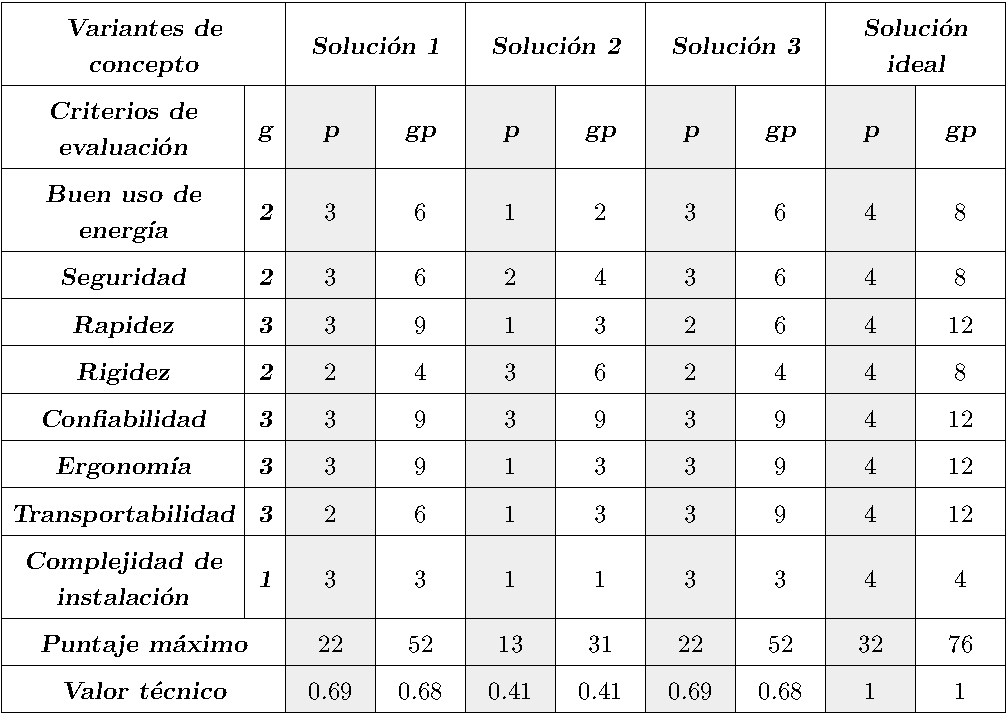
\includegraphics[width=0.95\linewidth]{eval_tec.pdf}
\end{table}

\newpage

\subsection{Evaluación económica}
\begin{table}[htbp!]
  \centering
  \caption{Evaluación económica}
  \label{diag:eval_econ}
  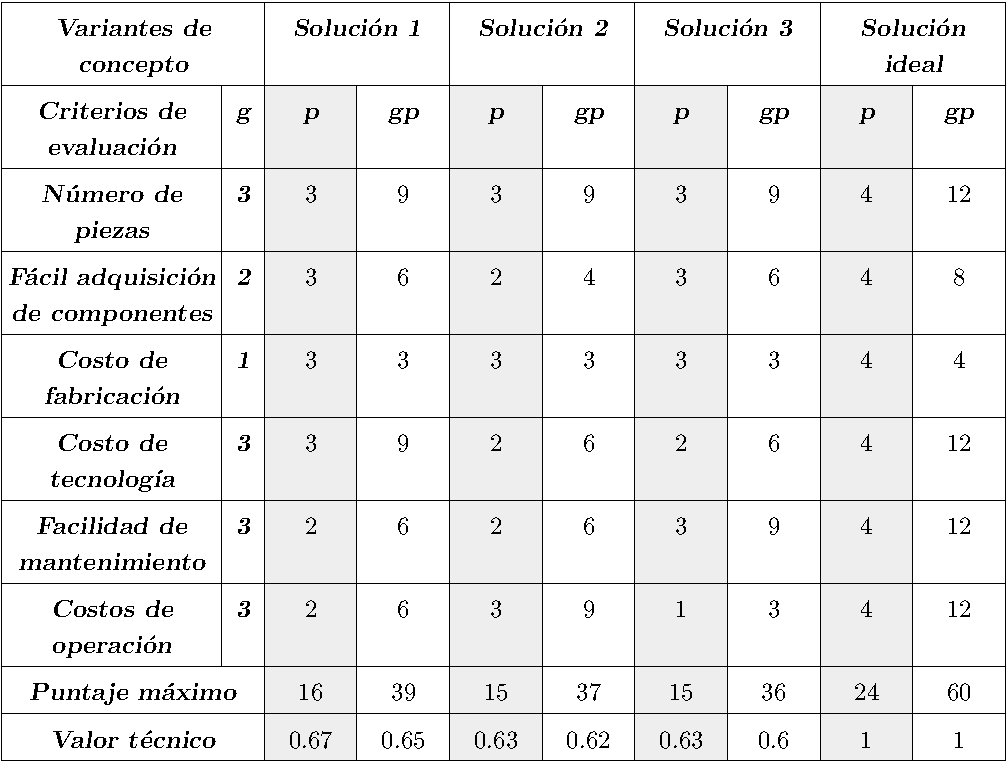
\includegraphics[width=0.95\linewidth]{eval_econ.pdf}
\end{table}

\subsection{Evaluación de soluciones}
\begin{figure}[htbp!]
\centering
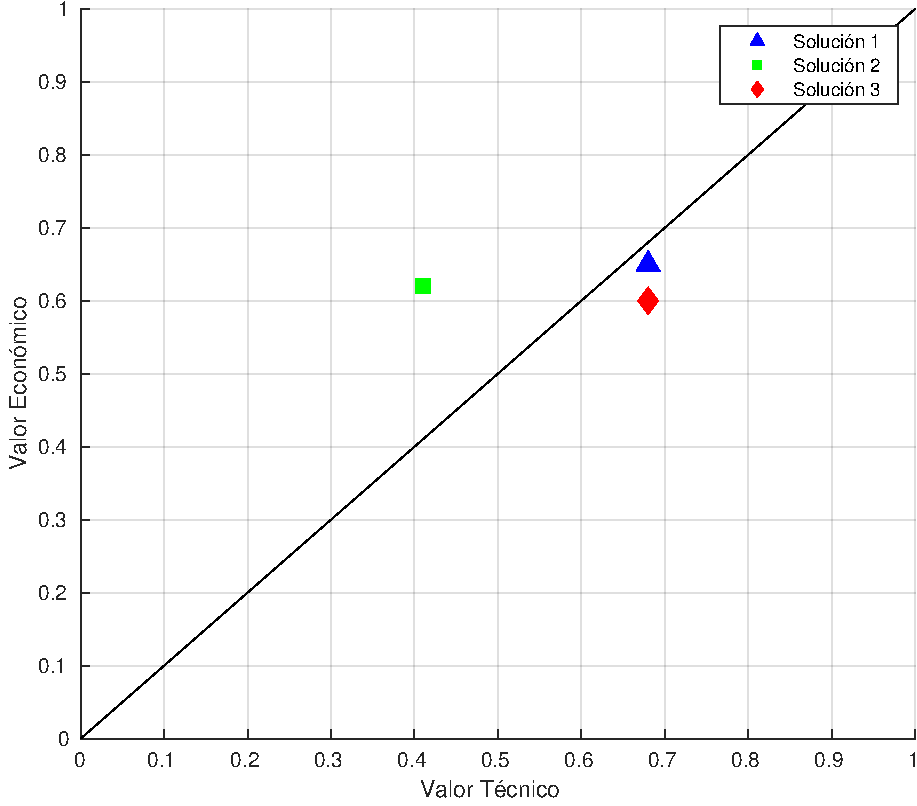
\includegraphics[width=0.8\textwidth]{grafico.pdf}
\caption{Diagrama de evaluación}
\label{diag:diag_eval}
\end{figure}

\begin{table}[htbp!]
  \centering
  \caption{Evaluación de soluciones}
  \label{diag:eval_sol}
  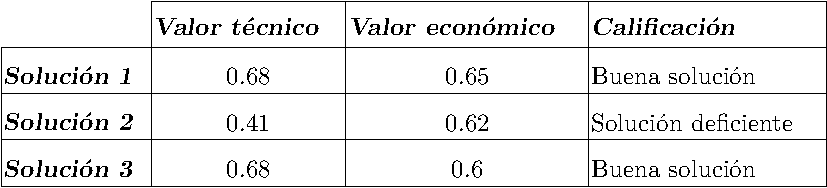
\includegraphics[width=0.9\linewidth]{tab_puntaje.pdf}
\end{table}

De acuerdo a lo observado en los análisis técnico y económico se consideran como buenas soluciones a las soluciones 1 y 3. Sin embargo, la solución 1 resulta la más adecuada. Por este motivo se escoge usar la solución 1 para el desarrollo de esta tesis.
